\subsection{Identifying the effects of a tactic: visual diffs}\label{peacoq-design-diffs}

Apart from terminators, which finish an obligation, most tactics will operate a
transformation on the goal of the current context.  The transformations can end
up changing entire types, or replacing sub-terms of some types with other terms.
Some tactics will also add hypotheses, remove some, or reorder hypotheses,
whether voluntarily or as part of how they need to operate.

In order for the user of a proof assistant to assess the usefulness of a
tactic's execution, they must be able to identify what changed by running the
tactic.  This is often done in a ad-hoc way, by going back and forth between the
state before and after the tactic, while visually inspecting differences.  This
is not satisfactory for several reasons.

First, finding out differences using this method is tedious.  Proof contexts
often contain dozens of variables and hypotheses, which makes the task of
finding the changes between two contexts both long, because the user might need
to repeatedly read several lines, and is error-prone, since the user might not
notice a change.

Second, \Coq{} does not offer great facilities for caching results, or viewing
results at a different proof context than the current one.  While rolling back
to the state prior to a tactic's execution is a fairly inexpensive action, due
to the \Coq{}'s state model, going back to the state after the tactic's
execution requires running the tactic again from scratch.  For slow tactics, the
process can be extremely slow, and while the tactic is running, the user might
forget about what they were looking for in the first place.

In order to have a better user experience, one would therefore need to be able
to inspect the state, before and after the execution of a tactic, without having
to run the tactic more than once.  Additionally, visual help indicating which
parts of the context have been modified could help accelerate finding the
effects of a tactic, while reducing the chances of missing a change or
mistakenly spotting a spurious change.

Fortunately, our proof-tree mechanism already provides us with a way of
displaying a before/after view of a proof context with respect to a tactic's
execution.  When a tactic is tried, but not committed to, we can display it as a
child of the current obligation node, and display its result as the child of
this tactic node.  By carefully aligning the two nodes, the user can have an
instant view of the two sides for comparison, without needing to run the tactic
ever again.  We cache those results so that the user can move in the tree
however they want.  Our trees are created in such a way that obligations nodes
have a unique execution history, such that when the user visits the same
obligation node, we can display the same tactic nodes, without needing to run
those tactics again.

We now introduce our notion of \define{visual diffs} as a means to highlight
changes between two proof contexts that are visually juxtaposed.  For a given
hypothesis in the original proof context, one of the following three outcomes
might happen to it as the result of a tactic execution: it may remain the same,
it may disappear, or it may by modified (either by being moved around, of by
having its name, term, or type changed).  Similarly, for a given hypothesis in
the final proof context, it may have originated from an unchanged hypothesis in
the original proof context, from a changed hypothesis in the original proof
context, or it may be a newly introduced hypothesis.

% TODO

\begin{figure*}[!htp]
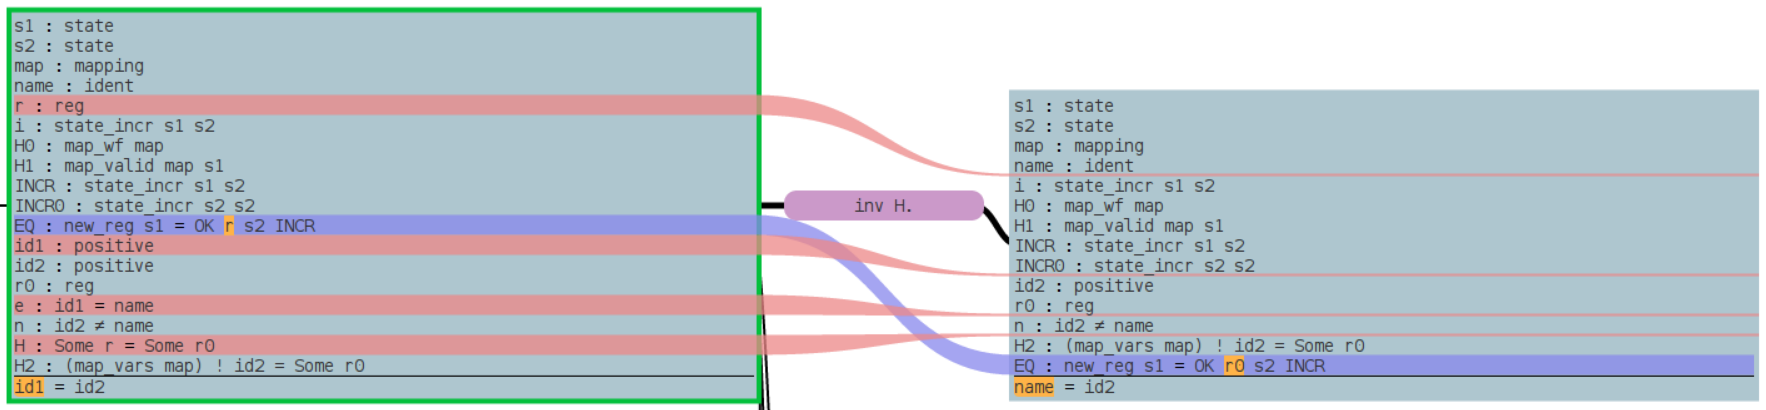
\includegraphics[width=\textwidth]{peacoq-diffs}{\parfillskip=0pt\par}
\caption{Proof-tree visual diff between two obligation nodes}%
\label{proof-tree-diffs}
\end{figure*}
